\documentclass[11pt,a4paper]{article}
\usepackage[hyperref]{latex/acl2021}
\usepackage{times}
\usepackage{graphicx}
\usepackage{latexsym}
\usepackage{amsmath}
\renewcommand{\UrlFont}{\ttfamily\small}
\usepackage[utf8x]{inputenc}
\usepackage{minted} 

% This is not strictly necessary, and may be commented out,
% but it will improve the layout of the manuscript,
% and will typically save some space.
\usepackage{microtype}

%\aclfinalcopy % Uncomment this line for the final submission
%\def\aclpaperid{2880} %  Enter the acl Paper ID here

%\setlength\titlebox{5cm}
% You can expand the titlebox if you need extra space
% to show all the authors. Please do not make the titlebox
% smaller than 5cm (the original size); we will check this
% in the camera-ready version and ask you to change it back.

\newcommand\BibTeX{B\textsc{ib}\TeX}

\title{\texttt{MaarX:} A Vocabulary of Mathematics from the ArXiv}

\author{Luis Berlioz\\
    University of Pittsburgh / \texttt{lab232@pitt.edu} }

\date{}

\begin{document}
\maketitle
\begin{abstract}
    We introduce ArGoT, a data set of mathematical terms extracted from 
the articles hosted on the arXiv website. 
A term is any mathematical concept defined in an article.
Using labels in the article's source code and examples from other
popular math websites, we mine all the terms in the
arXiv data and compile a comprehensive vocabulary of mathematical terms.
Each term can be then organized in a dependency graph by using
the term's definitions and the arXiv's metadata.
Using both hyperbolic and standard word embeddings, we demonstrate how 
this structure is reflected in the text's vector representation and
how they capture relations of entailment in mathematical concepts. This
data set is part of an ongoing effort to align natural mathematical
text with existing Interactive Theorem Prover  Libraries (ITPs) of
formally verified statements.
%% Include Formal abstracts project

\end{abstract}

\section{Introduction and Motivation}
Mathematical writing usually adheres to strict conventions of rigor
and consistent usage of terminology.
New terms are usually introduced in characteristically worded 
definitions (with phrases like \textit{if
    and only if} or \textit{we say a group is abelian...}). 
This feature can be used to train models to detect if a term is defined in a text.
%Also, the old 
%terms on which the new ones depend are seldom skipped.  
Using this, we have created \texttt{MaarX}, a silver standard data set of terms defined in
the Mathematical articles of the arXiv website.
We demonstrate that hyperbolic word embedding language models  
can effectively capture relations of entailment in advanced
mathematical concepts. Also, we show how standard models like word2vec
\cite{word2vec} and GloVe \cite{pennington2014glove} 
contain information that reflects the arXiv's metadata, like the
pertinence of term to a mathematical subject.
%And in the future, will provide abundant training examples for NLU and automated reasoning.
All these properties  make this a data set that will be of
interest to the broader NLP research community by providing abundant
examples for automated reasoning and NLU systems. The data is
downloadable from \texttt{[anonymized]} and the all the code that went
into producing it is in: \texttt{https://github.com/[anonymized]}
%the text with a unique predictability that enables the NLP researcher to perform
%adventurous experimentation and simple debugging.

%This data set was created  as part of the Formal Abstracts project.
%Our group has benefited from a grant from the Sloan  Foundation
%(G-2018-10067) and from the computing resources startup allocation
%\#TG-DMS190028 on the Bridges and \#TG-?? on the Bridges-2
%supercomputer at the Pittsburgh Supercomputing Center (PSC).

\begin{table}
    \small
\centering
\begin{tabular}{lr}
    \hline \textbf{Term} &  \textbf{Count} \\ \hline
lie algebra & 20524 \\
%suppose & 18043 \\
hilbert space & 16881 \\
function & 14920 \\
banach space & 14461 \\
metric space & 12882 \\
\_inline\_math\_-module & 12731 \\
topological space & 12518 \\
sequence & 12308 \\
disjoint union & 11436 \\
vector space & 11337 \\
simplicial complex & 10943 \\
graph & 10811 \\
map & 10654 \\
morphism & 10596 \\
\hline

\end{tabular}
\caption{\label{term-cnt-tab} Most common entries in the data base. }
\end{table}


\begin{table}
    \small
\centering
\begin{tabular}{lrrr}
    \hline
    \multicolumn{4}{c}{Classification Task} \\
    \hline
\textbf{Method}  & \textbf{Precision} &  \textbf{Recall} & \textbf{F1}\\ 
\hline
    SGD-SVM & 0.88 & 0.87 & 0.87 \\
    Conv1D & 0.92 & 0.92 & 0.92 \\
    BiLSTM & 0.93 & 0.93 & 0.93 \\
     \hline
    \hline
    \multicolumn{4}{c}{NER Task} \\
    \hline
    ChunkParse & 0.32 & 0.68 & 0.43 \\
    LSTM-CRF & 0.69 & 0.65 & 0.67 \\
    \hline
\end{tabular}
\caption{\label{metric-comp} Training metrics on the classification
    and NER tasks.}
\end{table}

\begin{table*}
    \centering
    \begin{minted}[fontsize=\small]{xml}
          <article name="1407_005/1407.2218/1407.2218.xml" num="89">
          <definition index="25">
            <stmnt> i. A function _inline_math_ is a weak solution 
            of problem (2.1) ... </stmnt>
            <dfndum>weak solution</dfndum>
          </definition>
          </article>
\end{minted}
\caption{\label{glossary-example} Example of an entry in the term's data set. Each entry contains all the information to recover, article's name and paragraph's position.}
\end{table*}

\section{Description of the Term-Definition Data Set}
In \citep{glossary, Deyan1}, the authors describe the 
method used  to obtain the training data for a text classification
model that identifies definitions and the (Named Entity Recognition) NER model that identifies the term being defined. 
The source of the training data is the source code of the \LaTeX{} 
articles, Wikipedia English dump and several mathematical websites like
PlanetMath\footnote{\url{https://planetmath.org/}} and The Stacks
Project\footnote{\url{https://stacks.math.columbia.edu/}}.

The classification task consist of training a binary classifier to determine whether a paragraph is a definition or not.  The definitions are then used by the NER task to identify the term being defined in them.
Following this approach we have compiled a data set by running the 
algorithm through all of the arXiv's mathematical content. 
Table \ref{term-cnt-tab} lists the most frequently found terms in the
data set. In table \ref{metric-comp} we list the methods that we
have tried on each task and the most common performance metrics. In
computing the NER metrics, we used the \texttt{ChunkScore} method in
the NLTK library \cite{bird2009natural}. 

The \texttt{MaarX} data set is distributed in the form of compressed
XML
files that follow the same naming convention the arXiv's bulk download
distribution\footnote{arXiv Bulk Data Access: \url{https://arxiv.org/help/bulk\_data}}.
For instance, table \ref{glossary-example} shows a sample entry
in the fifth file corresponding to July, 2014. The definition's
statement and definienda are specified in the \texttt{stmnt} and
\texttt{dfndum} tags respectively and the paragraph \texttt{index} is
specified as an attribute of the \texttt{definition} tag.

The data set contains 5,919,322 total entries with 1,007,769 distinct
terms. These values vary significantly depending on the model used to
collect them. Nonetheless, we have observed Cohen's kappa $\kappa$
\cite{cohenkappa} inter-rater
agreement of 93\% in the classification task between different methods.


%\begin{table}
\begin{figure}[h!]
    \small
\centering
\begin{tabular}{lc}
\hline
\textbf{Category:} & \textbf{Count}\\
\hline
math.FA& 5922 \\
 math.AP& 2045 \\
 math.PR& 1022 \\
 math.DS& 833 \\
 math.OA& 595 \\
 math.CA& 535 \\
 math.DG& 483 \\
 math-ph& 466 \\
 math.OC& 398 \\
 math.CV& 304 \\
 math.NA& 275 \\
 math.GR& 226 \\
 math.MG& 173 \\
 math.LO& 168 \\
 math.SP& 163 \\
math.NT& 131 \\
\hline
\end{tabular}
\begin{tabular}{lc}
\hline
\textbf{Category:} & \textbf{Count}\\
\hline
 math.GN& 108 \\
 math.RT& 85 \\
 math.SG& 77 \\
 math.GT& 76 \\
 math.CO& 61 \\
 math.ST& 61 \\
 math.KT& 50 \\
 math.GM& 48 \\
 math.AG& 35 \\
 math.RA& 33 \\
 math.HO& 32 \\
 math.CT& 23 \\
 math.AT& 15 \\
 math.QA& 10 \\
 math.AC& 8 \\
         & \\
\hline
\end{tabular}
\captionof{table}{Category profile for the term: \emph{Banach Space}. The codes
    are part of the metadata for each arXiv article.
}\label{tab:categories}
%\end{table}


%\begin{figure}[h]
%    \centering
    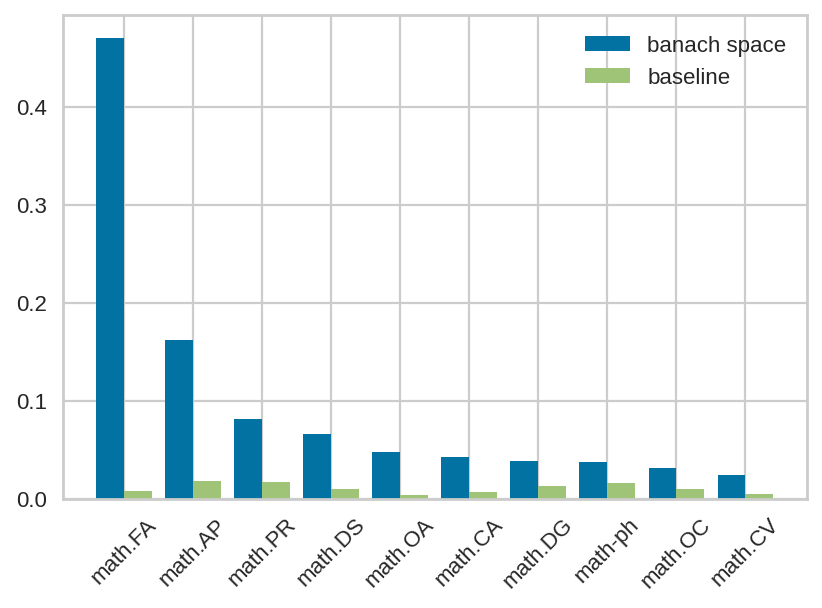
\includegraphics[width=0.5\textwidth]{images/barcomp.png}
    \captionof{figure}{\label{bar} Comparison between the term's category
        distribution and baseline distribution. Only categories with
        the highest values for the term are shown.}
\end{figure}

\section{Augmenting Terms with ArXiV's Metadata}
Each mathematical article in the arXiv is classified in one or more
\emph{categories} (see table \ref{tab:categories}) by the author at
the time of submission. In addition
to this, the arXiv also records information like the list of authors, math subject classification (MSC)~codes, date of submission and 
other metadata. 

By counting the categories in which a certain term is used, we get an
idea of the subjects that it belongs to. This is a feature of the arXiv's data that was not used at in either the classification or the NER tasks. In Table
\ref{tab:categories}, we see the category profile of a very common
term. Since the number of total articles in each category varies
significantly, we take into consideration the baseline distribution,
that is, the ratio of articles in each category to the total number of
articles.
Hence, it is possible to give an empirical score of a term's
pertinence to a certain category by comparing its category profile
with the baseline distribution. We then use the KL-divergence
%($D_{text{KL}}(P \Vert Q) = \sum_{x\in X} P(x)\log(P(x)/Q(x)$)
to measure how much of an outlier a term is to the baseline
distribution.
In fig.~\ref{scatter}, we observe a t-SNE (t-distributed stochastic
neighbor embedding) visualization of a word2vec 
model created using the arXiv math articles. For reasons of clarity,
in this figure we limited the number of categories to four and selected
15,000 terms with the highest (Kullback-Leibler) KL-divergence from the baseline out of the 100,000 most frequent terms. 

\begin{figure*}
    \centering
    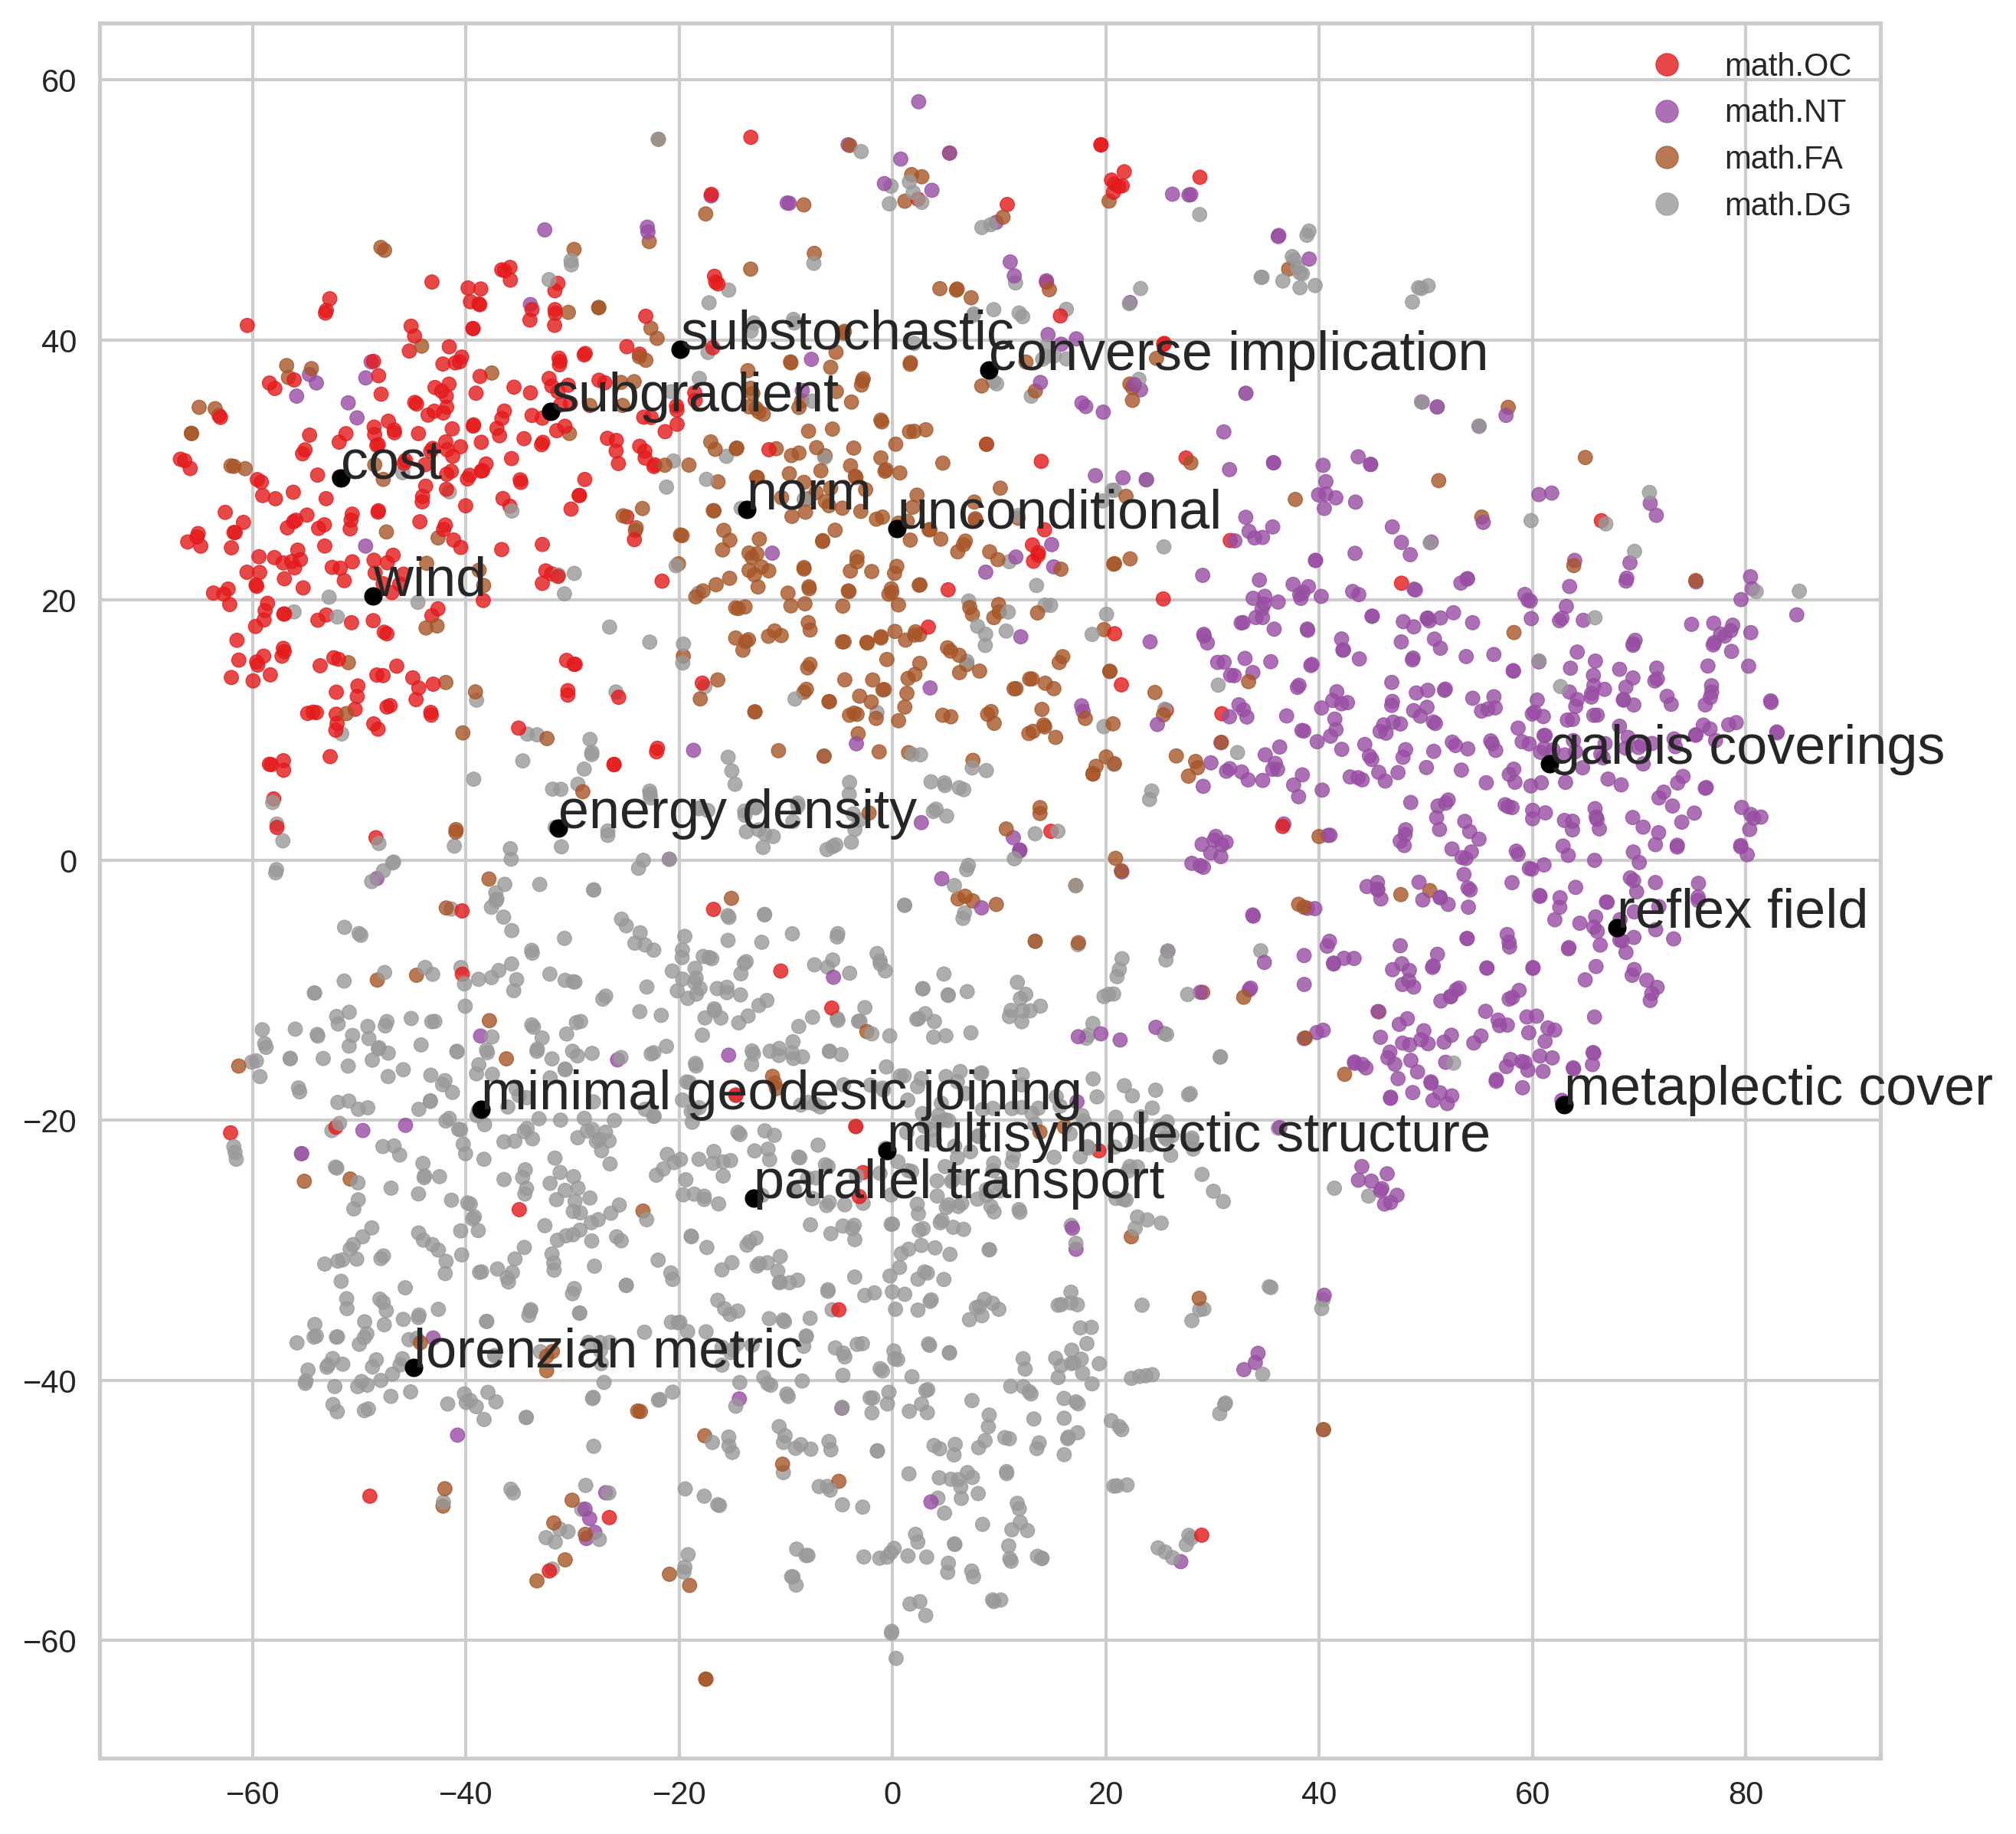
\includegraphics[width=0.7\textwidth]{images/scatter_option2.png}
    \caption{\label{scatter} TSNE visualization of the word vectors
        of selected terms in the data set. The terms are selected out
        of just 4 of the arXiv categories. Labeled points are selected
    at random.}
\end{figure*}
  



%\section{Distributed Representations and Semantic Evaluation}
\section{Distributed Representations with the arXiv's Content} 
We produced word embeddings of the arXiv in two rounds. The first one
was used in the classification and NER tasks, and the second one in
the embedding of joined terms. The source was processed in the
following ways: Substitute all math formulas, citations and
references with tokens, i.e. (\_inline\_math\_, \_cite\_, \_ref\_).
 Perform usual text normalization and tokenization for word 
embeddings. This includes removal of caps, numbers, non-ascii
characters, etc. In the second round,  Join the occurring instances 
of a term to create a unique token, for instance: \emph{banach space}
is joined as \emph{banach\textbf{\_}space}.
We produced both GloVe and word2vec word
embeddings and noticed no significant difference in performance.


%In order to perceive this property, 
%It is common for mathematical terms to be composed of multiple tokens.
%For instance, \emph{Riemann integral} and
%\emph{integral domain}. This means that detecting the multi-word entitiesis  necessary in order to take full advantage of mathematical text. 

\section{Using Hyperbolic Word Embeddings to Extract Hypernymy Relations}

We used PoincareGlove \cite{tifrea2018poincare} to create hyperbolic
word embeddings. This type of word embeddings is known to outperform
euclidean models in the representation of hierarchical structures \cite{facebookembeds}.

In order to evaluate the model, we produce a data set analogous to
WordNet \cite{wordnet}. In WordNet, every entry
is assigned an integer level in a hypernymy hierarchy (this is the
\texttt{max\_depth} attribute of the NLTK's WordNet
API\footnote{https://www.nltk.org/howto/wordnet.html}). Given two
term-definition pairs $(t_1, D_1)$ and $(t_2, D_2)$, we say that term
$t_2$ \emph{depends} on the term $t_1$ if $D_2$ contains $t_1$.  For
small sets of term-definition pairs with no interdependence, this
simple criterion is enough to create a directed graph $(V, E)$ where
$V$ is the set of all the terms and $E$ is the set of all the
dependency relations. To assign a level $\lambda (t)$ to every 
vertex $t\in V$, solve the following integer linear program:
\begin{align*}
    \text{min} & \quad \sum_{(v,w) \in E} \lambda(w) - \lambda(v)  \\
    \text{s.t.} & \quad \lambda(w) - \lambda(v) \geq 1  \\
     & \forall (v,w) \in E. 
\end{align*}
This idea was inspired by the directed graph drawing algorithm in 
\cite{graphsGasner}. 

Although the procedure above works for any term-definition data set,
we used data from the PlanetMath website, which is independent from 
the arXiv. 

Table \ref{tab:hypernyny} shows the nearest neighbors of four
different terms.  The neighbors are found using a word2vec model with
vectors of 500 dimensions that is completely independent of the
hyperbolic model used after. Also, for table \ref{tab:hypernyny}, we
used a 10 dimensional hyperbolic PoincareGlove model. The terms are 
sorted in order of the average value of their $y$-coordinates (which in
the upper-half plane model represents the variance of the underlying
Gaussian distribution).  


\begin{table}
    \small
\centering
\begin{tabular}{ll|ll}
    \hline \textbf{Term} &  $\mathbf{\sigma^2}$ &  
    \textbf{Term} &  $\mathbf{\sigma^2}$ \\ \hline
    hyperbolic\_metric & -1.11 &  &\\
euclidean\_metric & -0.59  & digraph & -0.51 \\
metrics & -0.58 & undirected\_graph & -0.35 \\
riemannian\_metric & -0.46  &  undirected & -0.20 \\
riemannian & -0.42  & \textbf{directed\_graph} &  0.0\\
riemannian\_manif & -0.40 & graph & 1.24 \\
curvature & -0.27  & & \\
\textbf{metric} & 0.0 & & \\
\hline
banach\_algebra & -1.11  & probability\_distr & -0.24 \\
normed\_space & -0.98 & \textbf{random\_variable} & 0.0 \\
banach\_spaces & -0.38 & expectation & 0.23 \\
banach & -0.29  & distribution & 0.46 \\
closed\_subspace & -0.25 & probability & 0.67 \\
\textbf{banach\_space} & 0.0 & & \\
norm & 0.79 & & \\

\end{tabular}
\caption{\label{tab:hypernyny} Cosine similar words sorted by the
    Gaussian variance ($\sigma^2$). The term in bold font is the
queried value.}
\end{table}


\section{Conclusions and Further Work}
We introduced \texttt{MaarX}, an comprehensive glossary of mathematics
automatically collected from the mathematical content on the arXiv website. 
Essentially, it is set of term-definition pairs, where 
each pair can be contextualized in a large semantic network of
mathematical knowledge, i.e., dependency graph. We also showed how this 
network is reflected in the latent space of its vector embeddings. This
has great potential for use in experimentation of natural language
algorithms, by providing a source of logically consistent data. 

This project is an ongoing effort to align mathematical concepts
in natural language with  online repositories of formalized
mathematics like
\texttt{mathlib}\footnote{https://github.com/leanprover-community/mathlib}. 

In the near future we plan to further improve on the classification 
and NER tasks by creating a data set using solely the neural version
of the classifier and NER model. Also,  by using state-of-the-art
methods like the masked transformer language model \cite{bert} to
further improve the results. 
We also plan to compile the complete dependency graph in one 
large graph database. 


%This type of domain specific data collection 
%and ontology population is becoming more commonplace as NLP models
%improve in performance. We hope this data set and will be helpful 
%to the researchers a similar project of 

\bibliographystyle{latex/acl_natbib}
\bibliography{article}
\end{document}
